% Task 3 — Region Clustering
% Northeast Megaregion Freight Network Design
% All throughput figures are in thousand short tons (ktons) unless otherwise noted.

\section{Task 3 — Demand Mapping and Region Clustering}

Task 3 partitions the 14-state Northeast study area into 50 logistics regions suitable
for regional hub placement. It proceeds in two stages: Task 3.1 constructs the freight
demand map and composite infrastructure overlay that guide clustering; Task 3.2 executes
a Simulated Annealing (SA) graph-partitioning algorithm to produce a demand-balanced,
spatially contiguous, and infrastructure-aligned partition of all 434 NE county-equivalent
units.

\subsection{Demand Mapping and Infrastructure Overlay (Task 3.1)}

\paragraph{Throughput computation.}
County-level freight demand is derived from the Task 1 O-D matrix
(\texttt{Data/Task1/raw.parquet}) after removing non-palletizable bulk commodities
(SCTG groups 10--14 coal and 15--19 gravel). Two distinct throughput metrics are computed
for each of the 434 NE counties:

\begin{itemize}
  \item \textbf{Activity throughput} — the bidirectional endpoint sum across all flow
        types (internal + inbound + outbound). Ranges from 25{,}180 ktons (minimum county)
        to 161{,}536 ktons (maximum county) at the region level after assignment. Used
        exclusively for choropleth visualization.
  \item \textbf{External throughput} — flows where exactly one endpoint is inside the NE
        and the other is outside. This is the hub-facing demand proxy: it captures only
        freight that must traverse a regional hub to enter or exit the megaregion. Used
        as the demand weight $W_i$ in the SA clustering objective.
\end{itemize}

This distinction is critical. Using activity throughput as a clustering weight would
double-count internal flows and inflate the demand-balance objective for large metro
counties. A post-assignment correction script further subtracts any remaining same-region
flows from the external throughput to produce fully corrected hub-facing demand metrics.

\paragraph{Composite map.}
County throughput centroids are joined to Census 2024 county boundaries
(EPSG:9311 projected coordinates) and overlaid with NTAD interstate highway segments
clipped to the 14-state area, Census TIGER railroad network lines, and the 29 Task 2
interface nodes (global, continental, and national tiers). The resulting composite map
(Figure~\ref{fig:task3-composite}) provides a visual synthesis of the freight intensity
landscape, corridor structure, and external gateway locations that collectively inform
subsequent clustering and hub placement decisions.

\begin{figure}[!ht]
  \centering
  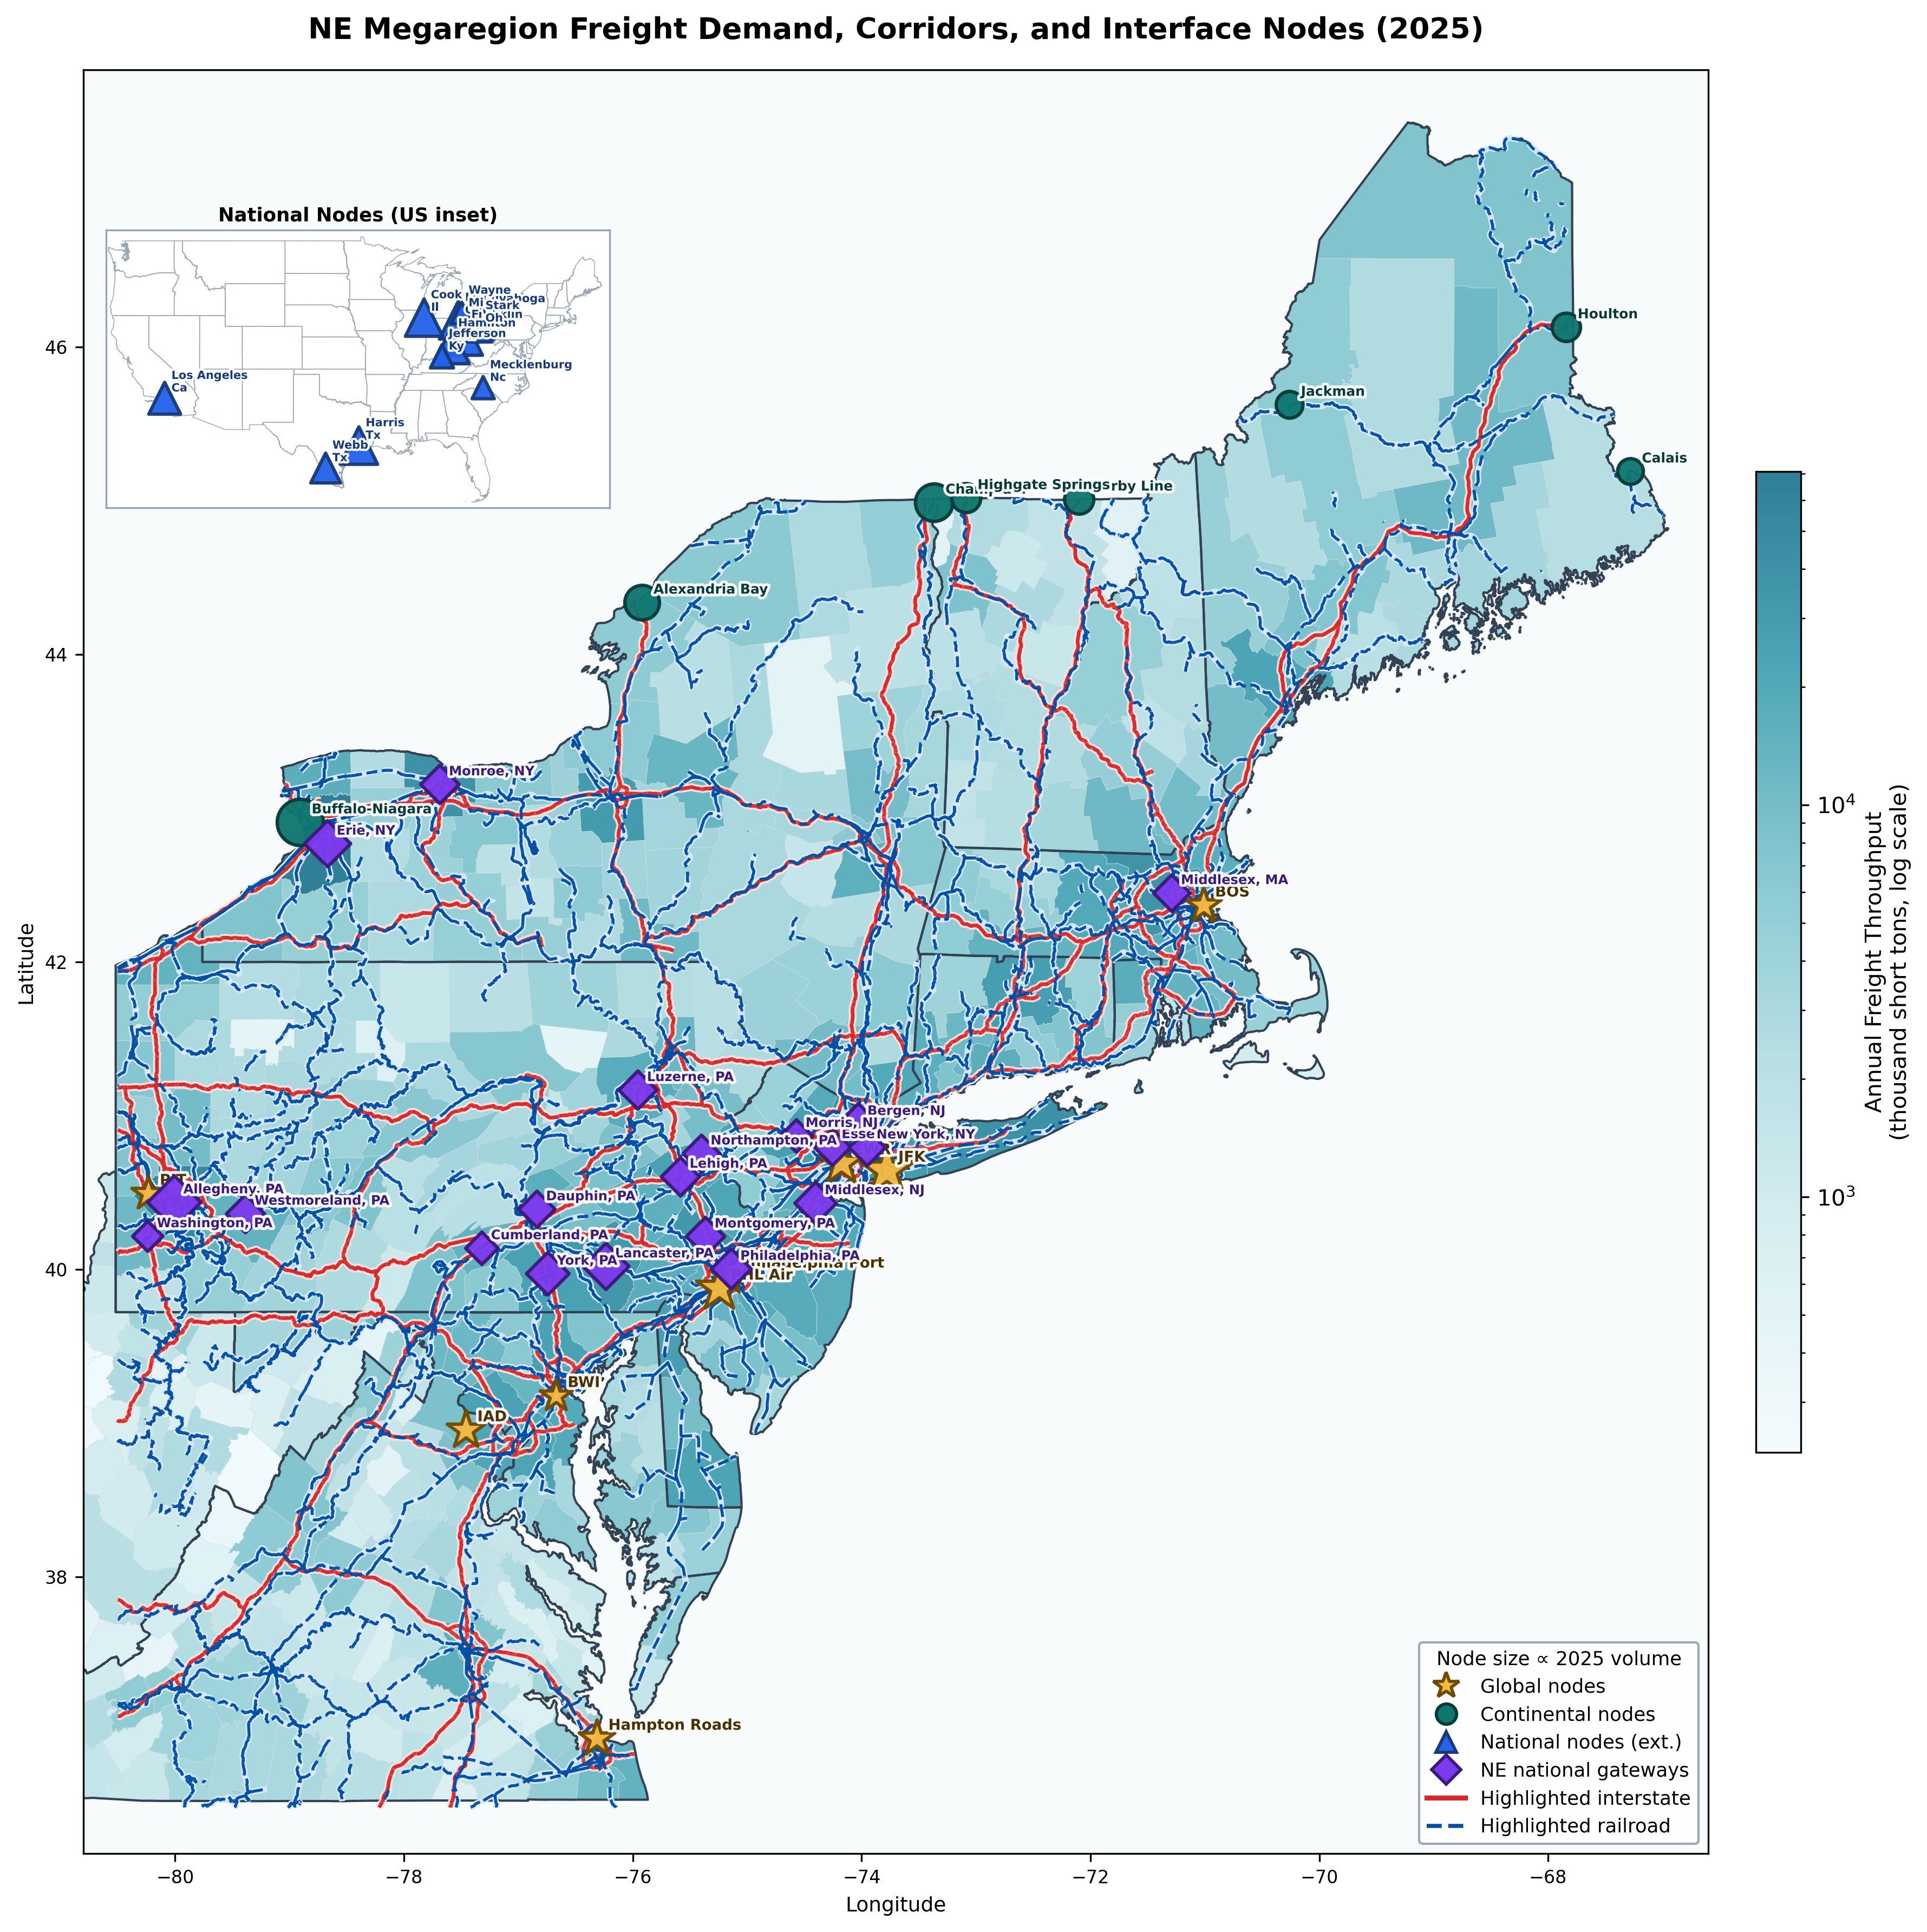
\includegraphics[width=0.85\textwidth]{figures/task3_composite_map.png}
  \caption{Composite freight demand and infrastructure map for the 14-state Northeast
    megaregion. County-level freight activity throughput is shown as a choropleth;
    NTAD interstate corridors (red) and rail lines (gray) are overlaid along with Task 2
    interface nodes. High-demand counties cluster along the I-95, I-78, and I-90
    corridors.}
  \label{fig:task3-composite}
\end{figure}

The demand heatmap (Figure~\ref{fig:task3-heatmap}) isolates the throughput intensity
signal, revealing that freight activity is heavily concentrated in the
Philadelphia--New York--Boston coastal corridor, Greater Pittsburgh, and the Albany--Buffalo
axis, with rapidly declining intensity in northern New England and West Virginia.

\begin{figure}[!ht]
  \centering
  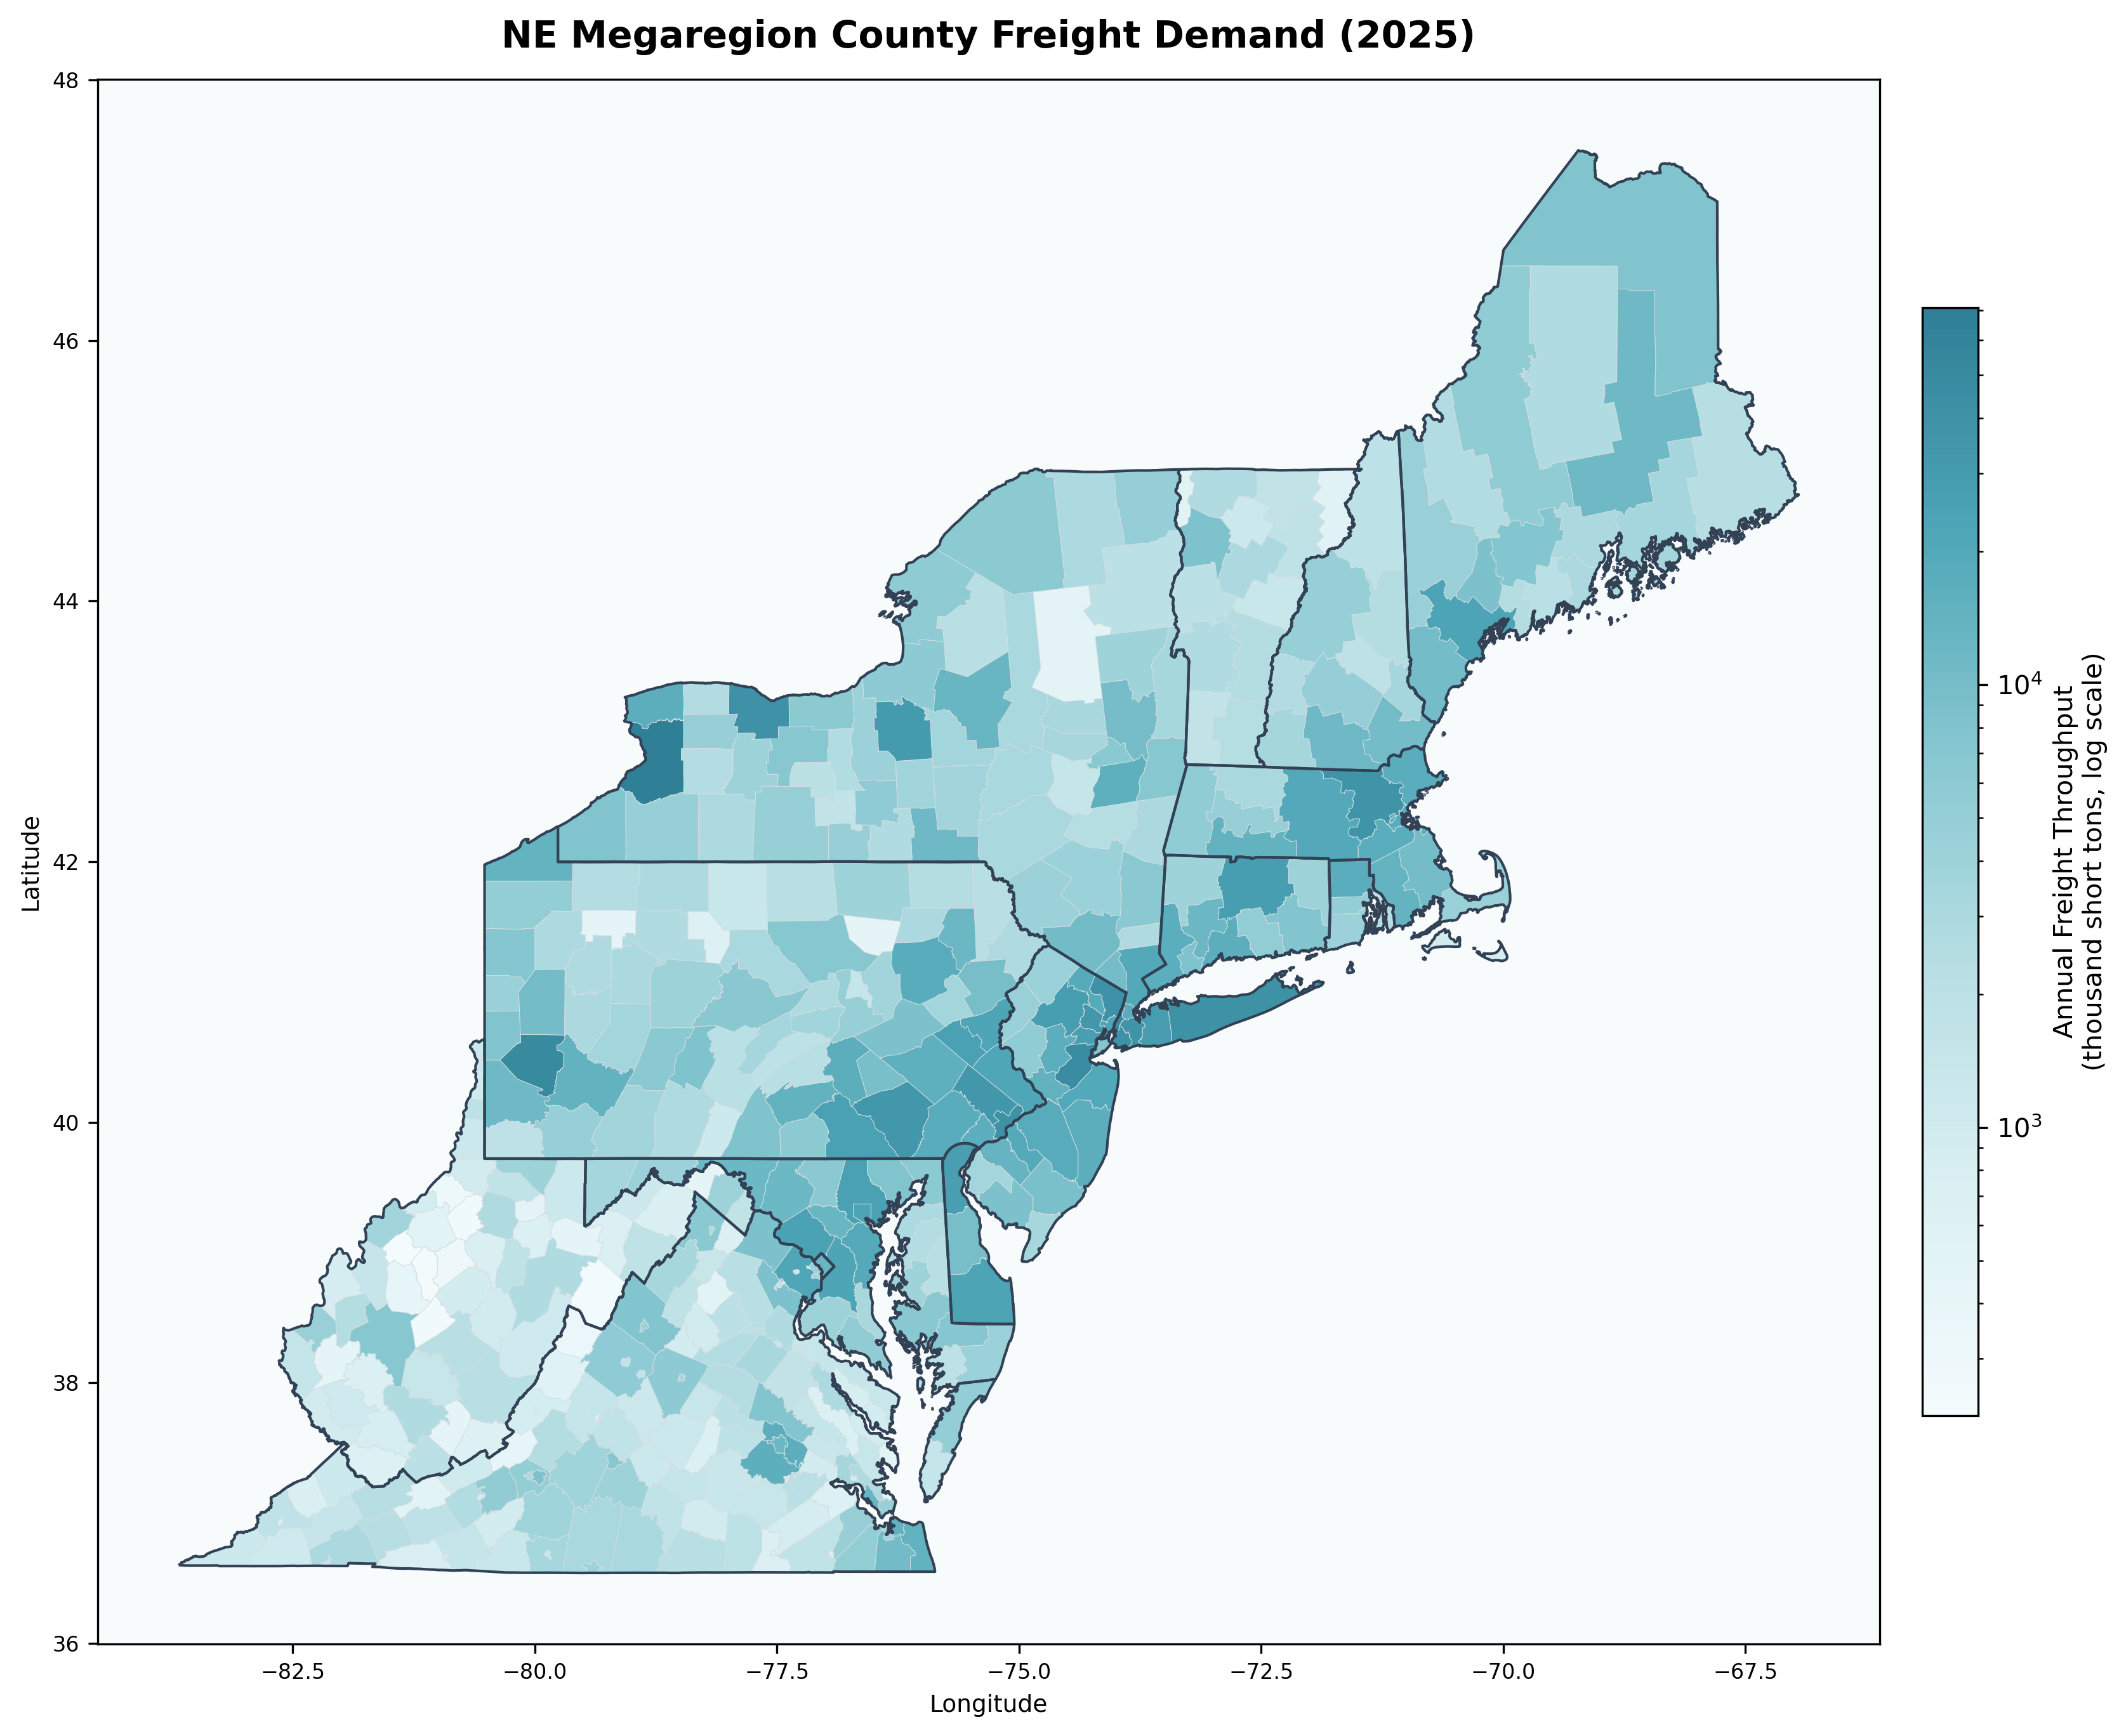
\includegraphics[width=0.85\textwidth]{figures/task3_demand_heatmap.png}
  \caption{County freight activity throughput choropleth (thousand short tons).
    The I-95 coastal belt and the Pittsburgh--Philadelphia corridor dominate the
    high-demand tier. Northern Maine, Vermont, and West Virginia exhibit the
    lowest throughput densities.}
  \label{fig:task3-heatmap}
\end{figure}

\subsection{Graph Construction and Adjacency}

The county adjacency graph $G = (V, E)$ is built over all 434 NE county-equivalent units.
Two counties share an edge if and only if they share a \emph{positive-length border
segment} (rook-style shared-border adjacency); point contacts are excluded. Known island
counties (e.g., Nantucket, Martha's Vineyard) receive synthetic links to their nearest
accessible mainland neighbors to ensure graph connectivity.

Each edge $(i, j)$ is attributed with:
\begin{itemize}
  \item \texttt{shared\_border\_m} — shared boundary length in meters,
  \item \texttt{interstate\_km} — total length of NTAD interstate segments crossing the
        shared border corridor,
  \item \texttt{rail\_km} — total length of TIGER rail segments crossing the corridor,
  \item \texttt{infra\_weight} — a normalized composite of interstate and rail coverage,
        used in the alignment objective.
\end{itemize}

The \texttt{infra\_weight} attribute encodes the importance of each edge to freight
corridor alignment: high values indicate that a border between two counties is crossed
by significant interstate or rail infrastructure and should therefore be \emph{preserved
within} a single region rather than cut.

\subsection{Simulated Annealing Formulation (Task 3.2)}

\paragraph{Problem statement.}
The clustering problem is to partition the set of 434 counties $V$ into $k = 50$
non-overlapping regions $\{R_1, \ldots, R_{50}\}$ such that each region is spatially
contiguous, the demand across regions is balanced, boundaries respect major freight
corridors, and regions are compact. Formally, the optimization minimizes a
three-component weighted objective $J$:

\begin{equation}
J = w_{\text{align}} \cdot C_{\text{align}} + w_{\text{compact}} \cdot C_{\text{compact}}
    + w_{\text{balance}} \cdot C_{\text{balance}}
\label{eq:task3-obj}
\end{equation}

where the three normalized components are:

\begin{align}
C_{\text{align}}   &= \frac{\displaystyle\sum_{(i,j)\in E} \omega_{ij} \cdot
    \mathbf{1}[r_i \neq r_j]}{\displaystyle\sum_{(i,j)\in E} \omega_{ij}}
    \label{eq:task3-align} \\[6pt]
C_{\text{compact}} &= \frac{1}{N \cdot D_0^2}
    \sum_{i \in V} \left\| (x_i, y_i) - (\mu_{x,r_i}, \mu_{y,r_i}) \right\|^2
    \label{eq:task3-compact} \\[6pt]
C_{\text{balance}} &= \frac{1}{k} \sum_{r=1}^{k}
    \left(\frac{W_r - W^*}{W^*}\right)^2
    \label{eq:task3-balance}
\end{align}

Here $\omega_{ij}$ is the infrastructure weight of edge $(i,j)$; $r_i$ is the region
assigned to county $i$; $D_0$ is the bounding-box diagonal of the study area (the
reference distance for compactness normalization); $W_r = \sum_{i \in R_r} W_i$ is the
total external throughput of region $r$; and $W^* = (\sum_i W_i) / k$ is the target
demand per region. The objective weights are set to $w_{\text{align}} = 1$,
$w_{\text{compact}} = 1$, and $w_{\text{balance}} = 4$, giving demand balance a 66.7\%
effective weight in the composite score — reflecting the primary requirement that regions
carry approximately equal freight volumes to avoid over- or under-sizing the regional
hubs.

All three components are unit-free by construction ($C_{\text{align}}$ is a fraction of
infrastructure-weighted cut edges; $C_{\text{compact}}$ is SSE normalized by $N D_0^2$;
$C_{\text{balance}}$ is mean squared relative deviation from target).

\paragraph{Hard constraints.}
Two move types are unconditionally rejected:
\begin{enumerate}
  \item \textbf{Contiguity}: the donor region $R_{\text{from}}$ must remain connected
        after removing the proposed county. This is checked via a breadth-first search
        (BFS) on the donor region subgraph.
  \item \textbf{Donor emptiness}: the donor region must retain at least one county.
\end{enumerate}

\paragraph{Incremental evaluation.}
The SA loop operates on $\Delta J$ rather than full $J$ recomputation. Each border-county
move affects only the two adjacent regions, so $\Delta C_{\text{align}}$ depends on the
neighborhood of the moved county; $\Delta C_{\text{compact}}$ depends on cached region
centroid statistics maintained in an $O(1)$-update \texttt{RegionStats} object;
and $\Delta C_{\text{balance}}$ requires only the throughput totals of the donor and
recipient regions. This design enables fast per-move evaluation without re-scanning the
full county set.

\subsection{Warm Start and Search Configuration}

\paragraph{Initialization.}
The SA warm start follows a two-phase procedure. First, weighted K-means ($k = 50$,
\texttt{n\_init=20}) is run on county projected centroids with external throughput as
sample weights to select 50 geographically dispersed seed counties. Second, a
demand-aware contiguous region-growing BFS assigns all remaining counties to their
nearest seed region, scoring candidates by a convex combination of distance-to-seed
($\alpha_{\text{dist}} = 0.5$) and demand-overshoot penalty
($\alpha_{\text{demand}} = 0.5$). This initialization produces a spatially valid
partition that is materially better than a random start, reducing the search burden on
the SA loop.

\paragraph{SA hyperparameters.}
The search is configured with the following parameters (Table~\ref{tab:task3-sa-params}):

\begin{table}[htbp]
\centering
\caption{Simulated Annealing hyperparameters for Task 3.2 region clustering.}
\begin{tabular}{ll}
\toprule
Parameter & Value \\
\midrule
Number of regions $k$ & 50 \\
Number of restarts & 4 \\
Proposals per restart & 15{,}000 \\
Total proposals & 60{,}000 \\
Cooling factor $\alpha$ & 0.9995 (geometric) \\
Initial temperature $T_0$ & Empirically sampled from $|\Delta J|$ distribution \\
Minimum temperature $T_{\min}$ & $10^{-6}$ \\
Early-stop patience & 5{,}000 proposals without improvement \\
Objective weights $(w_{\text{align}}, w_{\text{compact}}, w_{\text{balance}})$ & (1, 1, 4) \\
\bottomrule
\end{tabular}
\label{tab:task3-sa-params}
\end{table}

The initial temperature $T_0$ for each restart is sampled empirically by evaluating
$|\Delta J|$ on a random set of feasible border moves, then setting $T_0$ to the mean
$|\Delta J|$. This adaptive calibration ensures the acceptance probability for
worsening moves starts near 50\%, providing meaningful exploration before cooling
drives the search toward exploitation. Four restarts are executed; the best global
solution across all restarts is retained.

\begin{figure}[!ht]
  \centering
  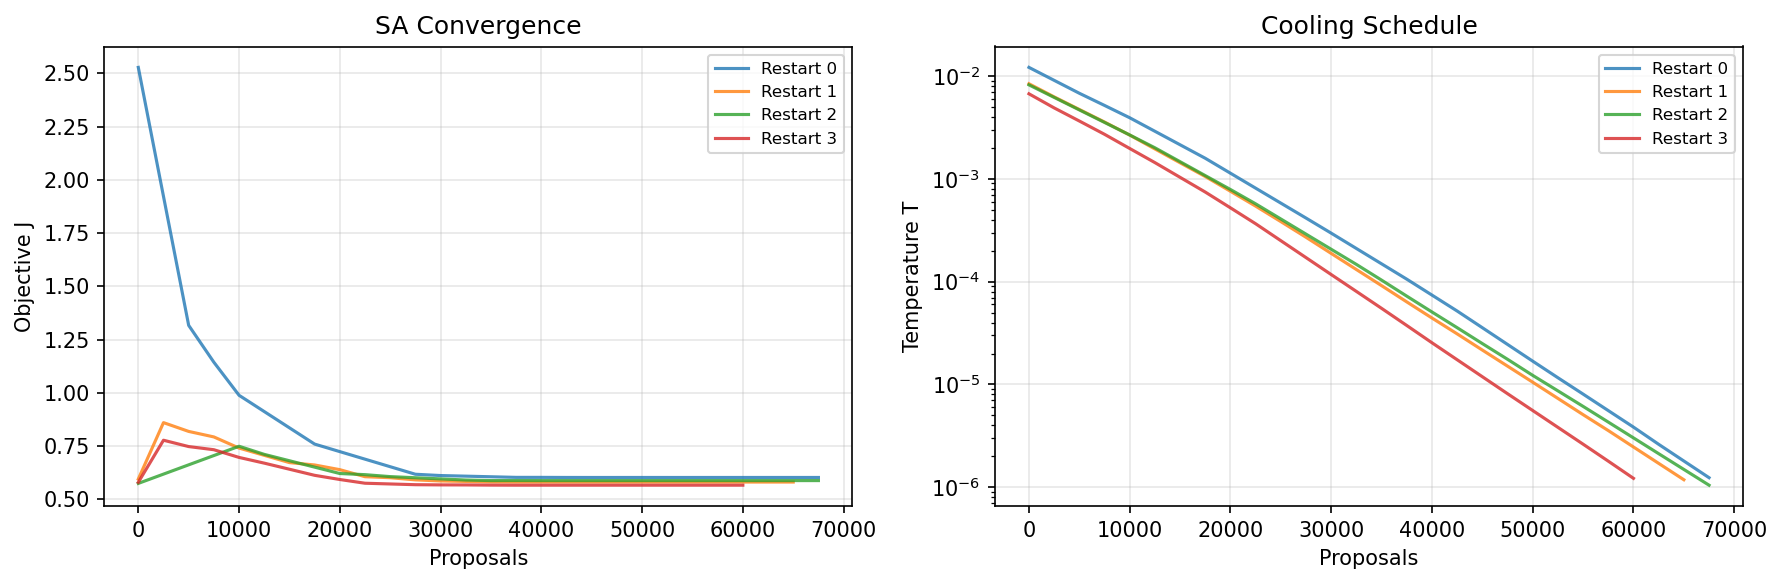
\includegraphics[width=0.65\textwidth]{figures/task3_sa_convergence.png}
  \caption{SA objective convergence across four restarts. The objective $J$ decreases
    from an initial value of 1.621 to a final best of 0.491, a reduction of 69.7\%.
    Each restart re-initializes temperature while retaining the best solution found,
    enabling continued refinement without losing prior gains.}
  \label{fig:task3-convergence}
\end{figure}

\subsection{Results and Quality Assessment}

The SA search ran for a total of 60{,}000 proposals across 4 restarts in approximately
20 seconds of wall-clock time. The convergence trajectory is shown in
Figure~\ref{fig:task3-convergence}. Table~\ref{tab:task3-quality} summarizes the
solution quality metrics.

\begin{table}[htbp]
\centering
\caption{Solution quality metrics for the final 50-region partition.}
\begin{tabular}{lr}
\toprule
Metric & Value \\
\midrule
Initial objective $J_0$               & 1.6205 \\
Final best objective $J^*$            & 0.4910 \\
Objective improvement                 & 69.7\% \\
Coefficient of Variation (CV)         & 0.230 \\
Normalized RMSE (nRMSE)               & 0.227 \\
Infrastructure-weighted cut fraction  & 0.320 \\
Spatially contiguous regions          & 50 / 50 \\
\midrule
Target demand $W^*$ (ktons)           & 8{,}947 \\
Min region demand (ktons)             & 7{,}043 \\
Max region demand (ktons)             & 19{,}766 \\
Mean region demand (ktons)            & 8{,}947 \\
Regions within $\pm$20\% of $W^*$    & 42 / 50 \\
Regions within $\pm$30\% of $W^*$    & 47 / 50 \\
\midrule
Total NE counties partitioned         & 434 \\
Mean counties per region              & 8.7 \\
Min counties per region               & 1 \\
Max counties per region               & 33 \\
\bottomrule
\end{tabular}
\label{tab:task3-quality}
\end{table}

The total external throughput across all 434 counties is 447{,}344 ktons, giving a
target $W^* = 8{,}947$ ktons per region. The final solution achieves a coefficient of
variation of 0.230, meaning most regions fall within roughly 23\% of the target demand.
Forty-two of 50 regions (84\%) lie within $\pm$20\% of $W^*$; 47 of 50 (94\%) lie within
$\pm$30\%. The notable outlier is region 7 at 19{,}766 ktons (121\% above target), which
corresponds to a large metro area whose demand cannot be further decomposed without
violating spatial contiguity. All 50 regions pass the contiguity check, confirming that
no isolated county groups exist in the final partition.

The infrastructure-weighted cut fraction of 0.320 indicates that 32\% of the total
infrastructure weight in the graph crosses region boundaries. A naive random partition
of equal-size regions would cut approximately 50\% of infrastructure weight; the SA
solution achieves meaningful corridor alignment by keeping major interstate and rail
corridors within single regions where feasible.

Figure~\ref{fig:task3-regions} shows the final 50-region map, with the demand balance
distribution displayed in Figure~\ref{fig:task3-balance}.

\begin{figure}[htbp]
  \centering
  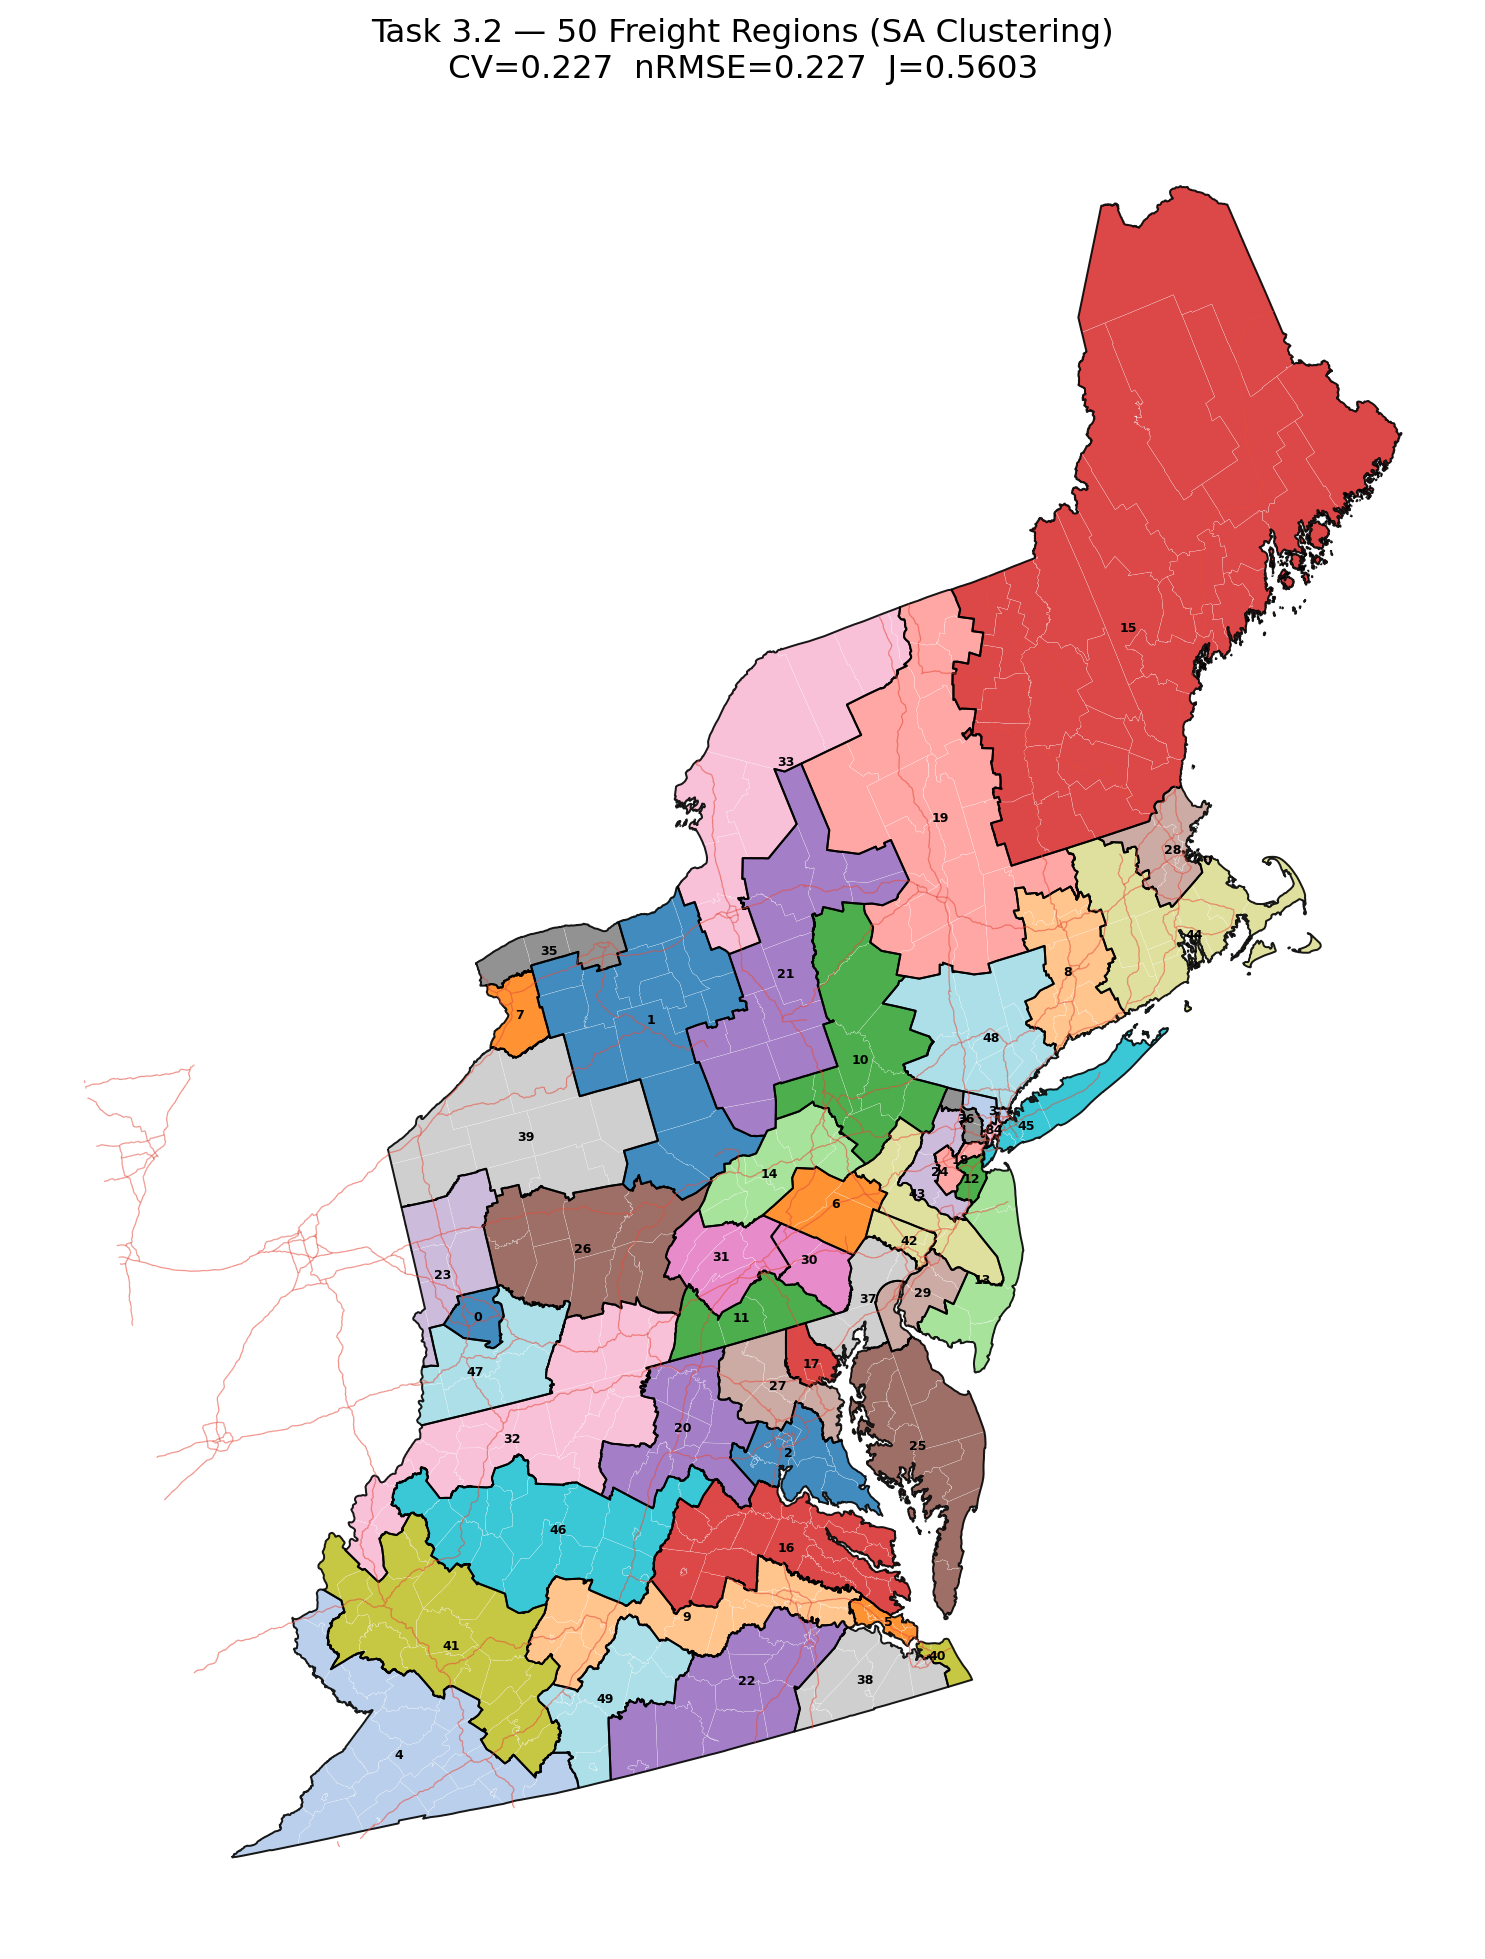
\includegraphics[width=0.85\textwidth]{figures/task3_region_map.png}
  \caption{Final 50-region partition of the 434-county Northeast megaregion.
    Regions are colored by identity. Major metro counties form dense, compact regions
    along the I-95 corridor; rural regions in northern New England and West Virginia
    aggregate many counties to reach the demand target.}
  \label{fig:task3-regions}
\end{figure}

\begin{figure}[htbp]
  \centering
  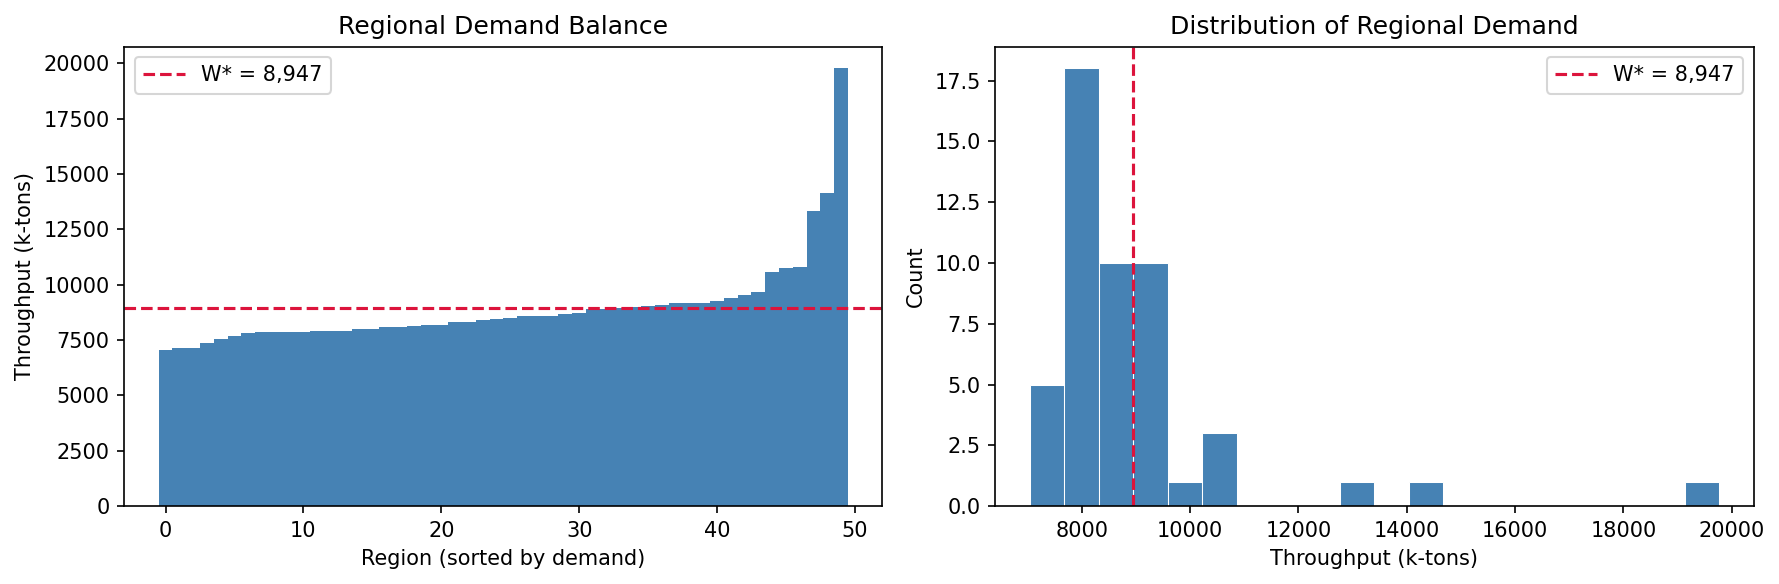
\includegraphics[width=0.65\textwidth]{figures/task3_demand_balance.png}
  \caption{Distribution of region-level external throughput relative to the target
    $W^* = 8{,}947$ ktons. The majority of regions cluster within 20\% of the target;
    a small number of high-demand metro regions exceed the target due to spatial
    contiguity constraints that prevent further subdivision.}
  \label{fig:task3-balance}
\end{figure}

The 50-region partition and associated county--region assignment table
(\texttt{region\_assignment.csv}) serve as the foundational territorial structure for
all downstream tasks: regional hub candidate screening (Task 5) uses region centroids
and demand weights to define coverage radii and size thresholds; area clustering (Task 6)
operates within each region; and the flow model (Task 8) routes freight through the
regional tier defined here.
